%!TEX encoding = UTF-8 Unicode

\documentclass[12pt]{scrartcl}

\usepackage{tikz}
\usepackage[utf8]{inputenc} % Unicode funktioniert unter Windows, Linux und Mac
\usepackage[T1]{fontenc}
\usepackage{ngerman}
\usepackage{graphicx}
\usepackage{amsmath}
\usepackage{times}
\usepackage[scaled]{helvet}
\usepackage{a4wide}
\usepackage{rotating}
\usepackage{hyperref}\urlstyle{rm}

\usepackage{listings}\lstset{breaklines=true,breakatwhitespace=true,frame=leftline,captionpos=b,xleftmargin=6ex,tabsize=4,numbers=left,numberstyle=\ttfamily\footnotesize,basicstyle=\ttfamily\footnotesize}
\sloppy
\setlength{\parindent}{0em}
\setlength{\parskip}{1.2ex plus 0.5ex minus 0.5ex}
\pagestyle{plain}

\begin{document}

\newpage

\thispagestyle{empty}
\begin{center}\Large
Universität Hamburg \par
Fachbereich Informatik
\vfill
Seminararbeit
\vfill
{\Large\textsf{\textbf{Funktionsweise der Honey Encryption}}\par}
\vfill
vorgelegt von 
\par\bigskip
Konstantin Kobs \par
geb. am 22. Februar 1993 in Geesthacht \par
Matrikelnummer 6414943 \par
Studiengang Informatik
\par\bigskip
Tom Petersen \par
geb. am 13. Dezember 1990 in Hannover \par
Matrikelnummer 6359640 \par
Studiengang Informatik
\vfill
eingereicht am \today
\vfill 
Betreuer: Prof. Dr.-Ing. Hannes Federrath \par
\end{center}

\newpage

\tableofcontents
\newpage

\section{Einleitung}

Auf der EUROCRYPT 2014 wurde von Ari Juels und Thomas Ristenpart ein neues Verfahren zur Absicherung von Verschlüsselung unter Nutzung von schwachen Schlüsseln (wie nutzergewählten Passwörtern) vorgestellt, das die Autoren in Anlehnung an bereits bestehende, ähnliche Systeme \emph{Honey Encryption} nennen. 

Das neuartige an diesem Verfahren ist, dass jede Entschlüsselung eines Ciphertexts unter einem zufälligen, nicht korrekten Schlüssel zu einer plausiblen Nachricht führt. Ein Angreifer, der keine weiteren Informationen über die Nachricht besitzt, kann die Nachricht so im Gegensatz zu bestehenden Verfahren nicht durch bloßes Ausprobieren aller möglichen Schlüssel knacken. Gerade nachdem in den letzten Jahren nach Angriffen auf Informationssysteme immer wieder Passwörter von Millionen von Nutzern bekannt geworden sind und Angreifern so relativ klare Vorstellung von der Passwortauswahl ermöglicht haben, ist Honey Encryption ein Fortschritt in der Sicherheit Passwort-basierter Verschlüsselung.

In dieser Seminararbeit soll das Honey Encryption-Verfahren näher beleuchtet werden. Dazu wird in dem Kapitel \ref{sec:funktionsweise} ein grober Überblick über heute verwendete Verfahren und ihre Schwächen gegeben und anhand eines Beispiels in die Funktionsweise und die notwendigen Einzelschritte der Honey Encryption eingegangen. Kapitel \ref{sec:dte} und \ref{sec:schema} erklären diese Einzelschritte dann ausführlicher und erläutern das Vorgehen auch anhand von konkreten Beispielen. In Kapitel \ref{sec:probleme} werden Einschränkungen betrachtet, die aus dem Verfahren selbst entstehen oder die bei seiner Verwendung betrachtet werden müssen.

Da das Verfahren erst vor kurzer Zeit vorgestellt und noch keine relevante Sekundärliteratur zu diesem Thema veröffentlicht wurde, folgt diese Arbeit in weiten Teilen der Argumentation von Juels und Ristenpart in \cite{EURO2014} bzw. \cite{IEEE2014}. 
\newpage
\newpage

\section{Notationen}

In den folgenden Abschnitten, in denen auf die Funktionsweise der Honey Encryption eingegegangen wird, werden folgende Notationen verwendet. Diese stimmen nicht vollständig mit der verwendeten Literatur überein.

\begin{tabular}{lp{14cm}}
\(\mathcal{M}\) & der Message Space, die Menge aller möglichen Nachrichten. \\ 
\(\mathcal{K}\) & der Key Space, die Menge aller möglichen Schlüssel. \\ 
\(\mathcal{C}\) & die Menge aller möglichen Ciphertexte. \\ 
\(\mathcal{S}\) & der Seed Space. Näheres dazu insbesondere in Abschnitt \ref{sec:dte}. \\ 
\(P(X)\) & die Wahrscheinlichkeit für das Eintreten des Ereignisses X.\\ 
\(\overset{<r>}{=}\) & eine nicht-deterministische Zuweisung. Dies kann entweder komplett zufällig geschehen (wie bei der Generierung von zufälligen Bitstrings) oder zumindestens vom Zufall mitbestimmt werden (wie bei der Kodierung einer Nachricht durch die DTE). \\ 
\(a \oplus b\) & die XOR-Verknüpfung von a und b. \\ 
\(S || T\) & die Konkatenierung der Zeichenketten S und T. \\ 
\(S{[1..n]}\) & die Nutzung der ersten n Zeichen von S. \\ 
\(\epsilon\) & die leere Zeichenkette. \\ 
\end{tabular}

\newpage

\section{Funktionsweise}
\label{sec:funktionsweise}

Honey-Objekte werden in der IT-Sicherheit in vielfacher Weise zum Aufdecken, Abwehren oder Untersuchen von Angriffen auf Systeme genutzt. Am bekanntesten dürften die Honeypots sein --- Server oder Programme, die Systeme simulieren, um Informationen über das Verhalten von Angreifern zu erlangen oder Einbrüche aufzudecken. Aber auch weniger bekannte Verfahren wie Honeydocuments, Honeyfiles oder Honeywords sind in diesem Bereich anzusiedeln. Grundsätzlich geht es hier darum, ein echtes Objekt zwischen Täuschungen (den Honey-Objekten) zu verstecken. 

All diese Verfahren verbinden zwei Eigenschaften: Ununterscheidbarkeit, d.h. Honey-Objekte sollten nur schwer vom echten Objekt differenzierbar sein, und Geheimhaltung, d.h. die bloße Kenntnis der Existenz von Honey-Objekten darf einem Angreifer auf das System keinen Vorteil bringen (frei nach dem Kerkhoffs'schen Prinzip: Nicht das Verfahren, sondern lediglich der Index des echten Objekts in der Liste aller Objekte ist geheim zu halten) \cite{SACMAT2014}.

In \cite{EURO2014} stellen die Autoren Honey Encryption vor --- ein neues Verfahren, welches die Nutzung von Honey-Objekten auf Passwort-basierte Verschlüsselung (\textit{Password-Based Encryption}, PBE) anwendet.

\subsection{Passwort-basierte Verschlüsselung und die Brute-Force Bound}

Grundsätzlich besteht ein PBE-Schema aus einer Verschlüsselungsfunktion \textit{Enc} und einer Entschlüsselungsfunktion \textit{Dec}. Eine Nachricht \(M\) wird mit einem Schlüssel \(K\) durch die Verschlüsselungsfunktion in den Chiffretext \(C\) überführt: \(\text{Enc}_K(M)=C\). Die Entschlüsselung erfolgt analog dazu: \(\text{Dec}_K(C)=M\). 

Ein Angreifer, der außer \(C\) keine weiteren Informationen besitzt, wird versuchen, per Brute-Force-Angriff (also durch rohes Durchprobieren aller möglichen Schlüssel) an die Nachricht \(M\) zu gelangen. Er wählt einen Schlüssel \(K' \in \mathcal{K}\) und bildet \(\text{Dec}_{K'}(C)=M'\). Durch die Nutzung von Authenticated Encryption (z.B. Encrypt-then-MAC, siehe \cite{AE2000}) erfährt der Angreifer sofort, ob er den richtigen Schlüssel gefunden hat. Bei diesen Verfahren wird schon vor der Entschlüsselung anhand eines Message Authentication Codes (MAC) überprüft, ob die verschlüsselte Nachricht nicht verändert wurde und der Schlüssel stimmt. Aber auch bei nicht authentifizierter Verschlüsselung lässt sich in den meisten Fällen leicht herausfinden, ob das versuchte Passwort \(K'\) korrekt war, also \(K'=K\) und damit auch \(M'=M\) gilt. Dies kann aus unterschiedlichen Gründen möglich sein. Beispielsweise sei bekannt, dass M natürlichsprachig ist. Dadurch könnten viele entschlüsselte Nachrichten gleich verworfen werden. Andere Gründe können ein zum Teil bekanntes Nachrichtenformat (z.B. offene Dateiformate oder feste Dateiheader) oder andere bekannte Eigenschaften sein (z.B. könnte bekannt sein, dass \(M\) eine Primzahl darstellt, ...). 

Dieser Brute-Force-Angriff wird dann zum Problem, wenn Schlüssel geringer Entropie\footnote{Die Entropie steht für den mittleren Informationsgehalt einer Nachricht. Wenn also ein Passwort häufig gewählt wird, so ist der Informationsgehalt und damit auch die Entropie des Passworts geringer, da es eher erwartet wird.} gewählt werden und Angreifer damit in vielen Fällen nur wenige Versuche benötigen, um den richtigen Schlüssel zu finden.\footnote{So erwähnt \cite{IEEE2014} beispielsweise den Diebstahl von 32 Millionen Klartext-Passwörtern von Kunden der Firma RockYou im Dezember 2009. Hierbei stellte sich heraus, dass in etwa einem Prozent der Fälle \emph{123456} als Passwort gewählt worden war und auch andere ähnlich schwache Passwörter häufig vertreten waren.} Durch Verfahren wie Salting (siehe \cite{Schneier2006}) oder mehrfache Anwendung beispielsweise von Hashfunktionen bei der Zwischenschlüsselgenerierung (vergleiche \cite{pbkdf2000}) lässt sich diese Art von Angriffen zwar verlangsamen, aber nicht aufhalten. Es lässt sich zeigen, dass eine PBE-verschlüsselte Nachricht mit Wahrscheinlichkeit \(\frac{q}{c \cdot 2^{\mu}}\) per Brute-Force entschlüsselt werden kann, wobei \(q\) für die Anzahl der Versuche, \(c\) als verfahrensabhängige Konstante und \(\mu\) für die Min-Entropie der Passwortverteilung \(p_k\) steht. Diese Wahrscheinlichkeit bezeichnet \cite{EURO2014} als \textit{Brute-Force Bound} und gibt weiterhin \(\mu<7\) für realistische Passwortverteilungen an. Diese Grenze ist selbst bei Erhöhung von \(c\) durch oben erwähnte Verfahren sehr gering.

Würde man weiterhin einen (in Rechenzeit und Speicherplatz) unbeschränkten Angreifer annehmen, so würde die Nachricht auf jeden Fall geknackt werden. Honey Encryption bietet hierfür eine Lösung an.

\subsection{Einführung in die Honey Encryption}
\label{sec:funktionsweise-beispiel}

\begin{quote}
\textit{"`HE is designed to produce a ciphertext which, when decrypted with any of a number of
incorrect keys, yields plausible-looking but bogus plaintexts called honey messages."'} \cite{EURO2014}
\end{quote}

Durch diese Eigenschaft kann ein Angreifer, der per Brute-Force-Angriff vorgeht, nie sicher sein, ob die in jedem Fall erhaltene, korrekt aussehende Nachricht wirklich die vorher verschlüsselte Nachricht \(M\) ist. Dies gilt selbst für unbeschränkte Angreifer und insbesondere auch für Schlüssel geringer Entropie. Es lässt sich zeigen (und die Autoren tun dies in \cite{EURO2014} für einige konkrete Anwendungsfälle), dass die Wahrscheinlichkeit, die Nachricht per Brute-Force-Angriff auf den Ciphertext \(C\) zu knacken, bei korrekter Implementation des Verfahrens (bis auf einen vernachlässigbaren Summanden) nicht größer ist als die Wahrscheinlichkeit, \(M\) durch Entschlüsselung von \(C\) mit dem Schlüssel \(K\text{*}\), der am wahrscheinlichsten in \(\mathcal{K}\) ist, zu erhalten. Dies entspricht auch in etwa der Wahrscheinlichkeit, mit Auswahl von \(M\text{*}\), der Nachricht mit der größten Wahrscheinlichkeit in \(\mathcal{M}\), die richtige Nachricht \(M\) erhalten zu haben. Diese Aussage lässt sich jedoch auch ohne Kenntnis von \(C\) treffen, also hat der Angreifer durch Kenntnis von \(C\) keinen Vorteil erlangt.

Ein kleines Beispiel soll nun die grundsätzliche Funktionsweise darstellen (Abbildung \ref{fig:Beispiel}). Angenommen, es soll der liebste RGB-Farbanteil verschlüsselt werden. Es sei bekannt, dass jeder zweite Mensch blau und jeder vierte jeweils rot oder grün am liebsten mag. Damit ist die Verteilung der Nachrichten \(p_m\) bekannt. Der erste Schritt besteht nun darin, den liebsten Farbanteil grün durch eine DTE (Distribution Transforming Encoder, näheres in Abschnitt \ref{sec:dte}) auf den sogenannten Seed Space \(\mathcal{S}\) abbilden\footnote{Abbildung ist hier nicht rein mathematisch zu verstehen, denn es handelt sich nicht zwingend um eine deterministische Relation.} zu lassen. Für grün erhält man so den Seed \(S=01\). Im zweiten Schritt wird S nun mit dem gewählten Schlüssel \(K=10\) XOR-verknüpft und es entsteht der Ciphertext \(C=01 \oplus 10 = 11\) (auf konkrete Verfahren zur Verschlüsselung wird in Abschnitt \ref{sec:schema} eingegangen).

\begin{figure}[!h]
\center
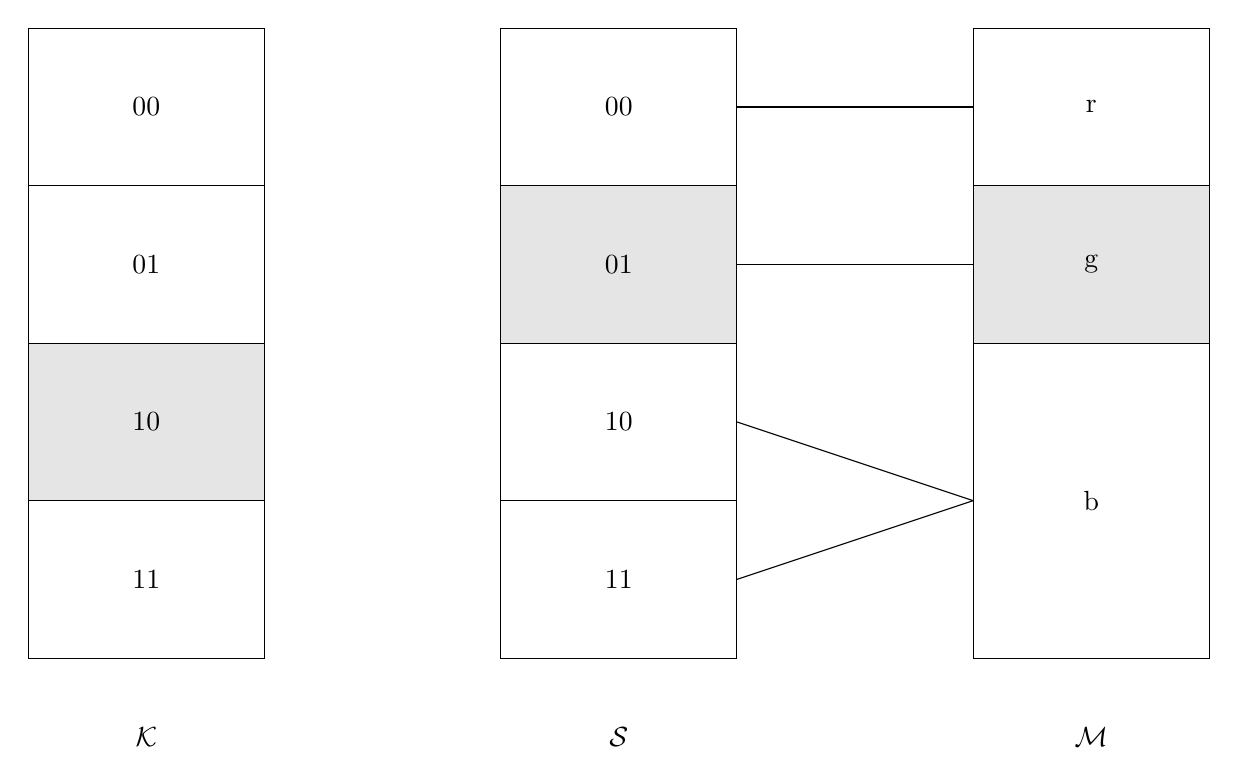
\begin{tikzpicture}
	% Linker Kasten
	\draw (1, 8) rectangle ++ (3, 2) node [midway] {$00$};
	\draw (1, 6) rectangle ++ (3, 2) node [midway] {$01$};
	\draw [fill=lightgray!40!white] (1, 4) rectangle ++ (3, 2) node [midway] {$10$};
	\draw (1, 2) rectangle ++ (3, 2) node [midway] {$11$};
	% Mittlerer Kasten
	\draw (7, 8) rectangle ++ (3, 2) node [midway] {$00$};
	\draw [fill=lightgray!40!white] (7, 6) rectangle ++ (3, 2) node [midway] {$01$};
	\draw (7, 4) rectangle ++ (3, 2) node [midway] {$10$};
	\draw (7, 2) rectangle ++ (3, 2) node [midway] {$11$};
	% Rechter Kasten
	\draw (13, 8) rectangle ++ (3, 2) node [midway] {r};
	\draw [fill=lightgray!40!white] (13, 6) rectangle ++ (3, 2) node [midway] {g};
	\draw (13, 2) rectangle ++ (3, 4) node [midway] {b};
	% Labels unten
	\node at (2.5, 1) {$\mathcal{K}$};
	\node at (8.5, 1) {$\mathcal{S}$};
	\node at (14.5, 1) {$\mathcal{M}$};
	% Linien
	\draw (10, 9) --++ (3, 0);
	\draw (10, 7) --++ (3, 0);
	\draw (10, 5) --++ (3, -1);
	\draw (10, 3) --++ (3, 1);
\end{tikzpicture}
\caption{Visualisierung des Beispiels}
\label{fig:Beispiel}
\end{figure}

Zur Entschlüsselung wird der Ciphertext \(C\) zunächst mit dem Schlüssel \(K\) XOR-verknüpft. Es entsteht der Seed \(S = 11 \oplus 10 = 01\). Dieser lässt sich nun von der inversen DTE wieder auf den liebsten Farbanteil abbilden und man erhältn wiederum grün. Ein Angreifer, dem nur \(C\) vorliegt, kann nun versuchen, den Farbanteil per Brute-Force herauszufinden. Dazu wählt er einen Schlüssel \(K'=00\) (beispielsweise, weil dieser am häufigsten verwendet wird) und bildet \(C \oplus K' = M' = 11\). Er erhält also blau. Ebenso gut hätte er rot oder auch grün erhalten können, aber in keinem Fall kann er sicher sein, die richtige Nachricht geknackt zu haben. Seine größte Erfolgswahrscheinlichkeit erhält er also dadurch, entweder \(C\) mit dem am häufigsten verwendeten Schlüssel zu entschlüsseln oder direkt die wahrscheinlichste Nachricht \(M\) (in diesem Fall also blau) anzunehmen.

\subsection{Unterschiede zu bestehenden Verfahren}

Um abgrenzen zu können, was Honey Encryption ausmacht, soll an dieser Stelle auf einige Verfahren eingegangen werden, die ähnlich arbeiten oder auf den ersten Blick ähnlich aussehen (die Beispiele sind entnommen aus \cite{EURO2014} und \cite{IEEE2014}).

Das erste Verfahren, das betrachtet werden soll, ist das sogenannte One Time Pad. Hierbei handelt es sich um simple XOR-Verknüpfung der Nachricht mit einem mindestens ebenso langen, zufälligen Schlüssel, der nur ein einziges Mal verwendet werden darf. Bei der Entschlüsselung lässt sich so je nach gewähltem Schlüssel jede andere (gleich lange) Nachricht mit gleicher Wahrscheinlichkeit erhalten. Bei dem One Time Pad handelt es sich jedoch nicht um ein Honey Encryption-Schema, denn erstens liefert die Entschlüsselung mit zufälligem Schlüssel nur in den wenigstens Fällen eine plausible Nachricht und zweitens werden auf jeden Fall Schlüssel hoher Entropie benötigt, Honey Encryption soll jedoch auch mit Schlüsseln geringer Entropie Sicherheit bieten.

Auch existierende AE- oder PBE-Schemata eignen sich, wie oben erklärt, nicht für die Honey Encryption, da die meisten entschlüsselten Nachrichten leicht als nicht plausibel verworfen werden können.

Als Letztes sei noch der Unterschied zu explizit gespeicherten Täuschobjekten erwähnt, wie sie beispielsweise in \cite{ACM13} verwendet werden. Bei diesen Verfahren werden neben der echten Nachricht \(n\) andere Honey Messages explizit gespeichert und (übertragen auf das hier betrachtete Gebiet) im Falle eines falschen Schlüssels bei der Entschlüsselung zurückgegeben. Im Gegensatz zur optimalen Honey Encryption ist die Erfolgswahrscheinlichkeit bei diesen Verfahren immer durch \(\frac{1}{n}\) beschränkt und unabhängig von der Entropie der Schlüsselverteilung. Außerdem haben diese Systeme einen Speicherbedarf von \(\mathcal{O}(n)\), Honey Encryption gelingt dies im Optimalfall mit einem Bedarf von \(\mathcal{O}(1)\).
\newpage

\section{DTE}
\label{sec:dte}
Die DTE, Abkürzung für \emph{distribution-transforming encoder}, dient zum Abbilden einer Nachricht $M$ aus dem Message Space $\mathcal{M}$ auf einen Seed $S$ aus dem Seed Space $\mathcal{S}$. Gleichermaßen soll sie die Möglichkeit bieten, von einem Seed auf die ursprüngliche Nachricht abzubilden. Eine DTE ist also ein Tupel von Algorithmen
$$DTE = (encode, decode)$$
wobei $encode$ einen meist randomisierten Algorithmus der Form $\mathcal{M} \rightarrow \mathcal{S}$ und $decode$ einen deterministischen Algorithmus der Form $\mathcal{S} \rightarrow \mathcal{M}$ beschreibt.

Ein DTE-Schema $(encode, decode)$ wird als \emph{korrekt} bezeichnet, wenn für jede Nachricht $M \in \mathcal{M}$, die mit $encode$ in den Seed Space $\mathcal{S}$ und mit $decode$ anschließend wieder in den Message Space $\mathcal{M}$ abgebildet wird, das Resultat wieder die ursprüngliche Nachricht $M$  ist. Formal kann dies geschrieben werden als
$$P(decode(encode(M)) = M) = 1 \qquad f.a. M \in \mathcal{M}$$
wobei P ein Maß für die Wahrscheinlichkeit für das in den Klammern stehende Ereignis ist.

Bei der Konstruktion einer DTE ist nicht nur dies zu beachten. Wichtig ist ebenfalls, die Verteilung der Wahrscheinlichkeiten der Nachrichten im Message Space zu kennen. Sie wird mit $p_m$ bezeichnet. Entsprechend dieser Wahrscheinlichkeiten wird einer Nachricht eine Anzahl von Seeds zur Kodierung zugewiesen. Je wahrscheinlicher eine Nachricht ist, desto mehr Seeds werden ihr zugewiesen.

Bei der Verschlüsselung einer Nachricht $M \in \mathcal{M}$ weist der Algorithmus $encode$ dieser Nachricht einen Seed entsprechend ihrer Wahrscheinlichkeit zu. Da es jedoch mehr als einen Seed zu einer Nachricht geben kann, handelt es sich bei $encode$ um einen randomisierten Algorithmus, der zufällig und gleichverteilt einen der möglichen Seeds auswählt. Da diese Kodierungs-Methode nicht deterministisch ist, handelt es sich bei $encode$ um keine Funktion oder Abbildung im mathematischen Sinne. Der Begriff \emph{Abbildung} ist dennoch eine passende Umschreibung für das Vorgehen zur Kodierung der Nachricht, mit einem Seed als Resultat.

Jede Nachricht kann also durch mehr als einen Seed dargestellt werden, allerdings verweist jeder Seed auf genau eine Nachricht (zu sehen in Abbildung \ref{fig:dte}).

\begin{figure}[!h]
Seed Space und Message Space anzeigen und Pfeile einmalen
\caption{Relationen zwischen $\mathcal{M}$ und $\mathcal{S}$}
\label{fig:dte}
\end{figure}

Somit ist leicht zu erkennen, dass es sich bei $decode$ um einen deterministischen Algorithmus handelt. Der Begriff \emph{Abbildung} wäre in diesem Fall auch mathematisch korrekt.

Wie schon beschrieben, sollte
$$\frac{|\mathcal{S}_M|}{|\mathcal{S}|} \approx p_m(M) \qquad f.a. M \in \mathcal{M}$$
gelten, wobei $\mathcal{S}_M$ die Menge aller zu $M$ gehörenden Seeds und $p_m(M)$ die Wahrscheinlichkeit für die Nachricht $M$ ist. Die Verteilung, die sich durch $\frac{|\mathcal{S}_M|}{|\mathcal{S}|} \quad f.a. M \in \mathcal{M}$ ergibt, wird mit $p_d$ bezeichnet --- das $d$ im Index steht für \emph{distribution}, genau genommen die Verteilung, die durch die DTE ensteht.

Für eine gute DTE gilt also $p_d = p_m$.

\textbf{HIER SOLLTE WAHRSCHEINLICH NOCH ETWAS STEHEN, MUSS MAN SCHAUEN, IN WIE WEIT DAS OBERHALB HIERVON STEHENDE IN ALLGEMEINES KOMMT.}

\subsection{Generierung einer DTE mithilfe der Inversionsmethode}

Ein mögliches Vorgehen zur Erstellung einer DTE, die von Juels und Ristenpart \cite{EURO2014} vorgeschlagen wird, ist die Nutzung der sogenannten Inverse Sampling Methode, zu Deutsch Inversionsmethode. Sie wird in der Informatik und Stochastik angewendet, ``um aus gleichverteilten Zufallszahlen andere Wahrscheinlichkeitsverteilungen zu erzeugen.'' \cite{WIKIInv} Meist wird dieses Verfahren in der Informatik für die Simulation von Zufallsvariablen, wie beispielsweise dem Monte-Carlo-Verfahren, verwendet. Dabei wird einer Rechteckverteilung $R(0,1)$ eine neue Wahrscheinlichkeitsverteilung zugewiesen. So kann ein Computer Zufallszahlen erzeugen, die in einer beliebigen, neuen Verteilung liegen, als die normalerweise von ihm generierbaren Zahlen im Intervall $[0,1)$.

Wie schon beschrieben wurde, muss für die Generierung einer DTE $p_m$, also die Wahrscheinlichkeitsverteilung für die Nachrichten des Message Spaces, bekannt sein. Nach den Regeln der Stochastik hat jede Nachricht eine Wahrscheinlichkeit im Intervall $(0,1)$, wobei die Summe aller Wahrscheinlichkeiten gleich $1$ sein muss. Es sei hier explizit darauf hingewiesen, dass die Intervallränder $0$ und $1$ als Wahrscheinlichkeiten für Nachrichten ungeeignet sind. Gilt nämlich für eine Nachricht $M \in \mathcal{M}$ $P(M) = 0$, dann ist das Vorkommen dieser Nachricht nicht möglich und sollte somit gar nicht beachtet werden. Ein Vorkommen im Message Space ist damit überflüssig. Gilt andererseits für $M$ $P(M) = 1$, so ist dies die einzig mögliche Nachricht. Dann ist es nicht sinnvoll, Honey Encryption zu verwenden, da ein potentieller Angreifer zum eindeutigen Entschlüsseln nicht einmal den Ciphertext kennen müsste. Der Angriff wäre trivial.

Eine DTE wird mit diesem Vorwissen nun wie folgt erstellt: Es wird die Verteilungsfunktion $F_m$ der Verteilung $p_m$ genutzt. Gegeben sei dafür eine Ordnung der Nachrichten im Message Space $\mathcal{M} = \{M_1, \dots, M_{|\mathcal{M}|}\}$. Die Verteilungsfunktion einer Nachricht $F_m(M_i)$ ist nun die Summe der Wahrscheinlichkeiten der ersten $i$ Nachrichten.

$$F_m(M_i) = \sum_{k = 1}^{i} P(M_k)$$

Um die Grenzen festzulegen, sei $F_m(M_0) = 0$ und logischerweise $F_m(M_{|\mathcal{M}|}) = 1$. Eine Visualisierung für eine Verteilungsfunktion solcher Art ist in Abbildung \ref{fig:Verteilungsfunktion} zu sehen.

\begin{figure}[!h]
Visualisierung
\caption{Eine Visualisierung einer Verteilungsfunktion $F_m$}
\label{fig:Verteilungsfunktion}
\end{figure}

Sei nun der Wertebereich aller Seeds $S \in \mathcal{S}$ das Intervall $[0,1)$. Ein Seed $S$ wird dann in seine Ursprungsnachricht zurückgeführt (\emph{decode}-Algorithmus), indem die Nachricht $M_i$ gefunden wird, für die $F_m(M_{i-1}) \leq S < F_m(M_i)$ gilt. Wenn als Beispiel der Seed zwischen der Summe der ersten 5 und 6 Nachrichtenwahrscheinlichkeiten liegt, dann gibt der \emph{decode}-Algorithmus als ursprüngliche Nachricht zurück. Eine anders geschriebene und leichter in Programmen umsetzbare Schreibweise der Übersetzung von Seed in Nachricht ist

$$min_i\{F_m(M_i) > S\}$$

Anschaulich sei ein Maßband der Länge 1 betrachtet, auf der die Nachrichten entsprechend ihrer Wahrscheinlichkeiten aufeinanderfolgend und disjunkt aufgetragen (Abbildung \ref{fig:decode}) wurden. Ein Seed liegt nun irgendwo auf der Länge des Maßbandes. An dieser Stelle liegt auch eine Nachricht $M_i$, die dann als ursprüngliche Nachricht ausgegeben wird. Liegt der Seed dabei auf der Grenze zweier Nachrichten, wird die weiter rechts liegende zurückgeliefert.

\begin{figure}[!h]
Maßband mit Nachrichten und 0 links und 1 rechts
\caption{Eine anschauliche Darstellung des \emph{decode}-Algorithmus}
\label{fig:decode}
\end{figure}

Es ist an der anschaulichen Darstellung unschwer zu erkennen, dass die Verteilung $p_m$ in der DTE wieder zu finden ist. Die Wahrscheinlichkeit einer Nachricht wird durch ihre Breite dargestellt. Da die Seeds gleichverteilt sind, ist es leichter, einen besonders breiten Abschnitt zu treffen, als einen schmaleren.

Bisher wurde der \emph{decode}-Algorithmus betrachtet. Der \emph{encode}-Algorithmus ist ähnlich anschaulich zu erklären. Dieses Mal wird eine Nachricht gewählt, die auf dem Maßband liegt. Der Bereich an Werten auf dem Maßband, der von dieser Nachricht abgedeckt wird, wird als Grundlage für eine Auswahl eines Seeds verwendet. Dabei wird zufällig gleichverteilt ein Wert aus diesem Bereich ausgewählt.

Auf die Verteilungsfunktion bezogen ist ein Seed, der aus der Nachricht $M_i$ generiert wird, eine reelle Zahl im Intervall $[F_m(M_{i-1}), F_m(M_i))$. Die Auswahl aus diesem Intervall lässt sich mithilfe eines Computers recht einfach bewerkstelligen, da dieser im Normalfall reelle Zufallszahlen im Intervall $[0,1)$ generieren kann.

Auch hier ist klar, dass es mehr mögliche Seeds für eine Nachricht geben kann, je wahrscheinlicher diese Nachricht ist. In diese Richtung ist die Eigenschaft einer guten DTE ebenfalls gegeben.

Um die erzeugte DTE praktisch anwenden zu können, muss noch das Problem der Übersetzung der stetigen Werte zwischen $[0,1)$ in die diskreten Werte von in Binärzahlen angegebenen Seeds des Seed Spaces, welcher tatsächlich verwendet wird. Die Anzahl der Seeds sollte so gewählt werden, dass die Abweichungen der relativen Seed-Bereiche einer Nachricht in beiden Repräsentationen möglichst klein sind. Je größer die Abweichungen nämlich sind, desto mehr verzerrt sich die Verteilung der DTE. Die erstrebenswerten Eigenschaften einer guten DTE wären damit nicht mehr gegeben und es könnte zu einem Sicherheitseinbruch der Honey Encryption mit dieser DTE kommen.

\newpage
\newpage

\subsection{Eine DTE für private RSA-Schlüssel}

Das folgende Beispiel ist entnommen aus \cite{EURO2014}.

Bei RSA handelt es sich um einen asymmetrischen Verschlüsselungsalgorithmus, d.h. das Verfahren beruht auf einem öffentlichen und einem privaten Schlüssel. Zur Generierung der Schlüssel (heutiger Stand: 2000 Bit \cite{BSI2014}) wählt man zwei große  Primzahlen \(p\) und \(q\) und errechnet aus ihnen öffentlichen und privaten Schlüssel (zu Details siehe \cite{Schneier2006}). RSA wird beispielsweise bei SSL/TLS oder SSH eingesetzt. Für die Anwendung von Honey Encryption ist jedoch nur der zweite Fall geeignet, denn bei SSL/TLS ist der öffentliche Schlüssel des Servers bekannt und so ließe sich leicht nachprüfen, ob der richtige private Schlüssel entschlüsselt wurde. 

Bei SSH lässt sich Honey Encryption jedoch anwenden. In diesem Fall wird der öffentliche Schlüssel zum Zweck der Authentifizierung auf dem Server gespeichert, den man erreichen möchte (und steht somit dem Angreifer nicht zur Verfügung). Der private Schlüssel (genauer \(p\) und \(q\) zusammen mit weiteren berechneten Werten, um die Ver- bzw. Entschlüsselung nach dem Chinesischen Restsatz zu erleichtern) wird verschlüsselt auf dem Clientsystem gespeichert.

Zur Erstellung einer DTE für RSA-Schlüssel muss betrachtet werden, wie die Primzahlen \(p\) und \(q\) (im Folgenden werden Primzahlen aus dem Intervall \([2^{l-1},2^l)\) gefordert) erhalten werden. Normalerweise werden zufällige Zahlen aus dem Intervall gewählt und durch einen Primzahltest (z.B. Miller-Rabin-Test) auf Primzahleigenschaften hin überprüft. Dies wird solange wiederholt, bis man zwei Primzahlen gefunden hat. 

% Guck nochmal nach, wieso l-2
Ein naiver Ansatz für eine DTE wäre es, die beiden gefundenen Primzahlen als \((l-2)\)-Bitstrings zu dekodieren (die auf jeden Fall vorhandene führende 1 ist implizit und wird ausgelassen). Da jedoch bei der Entschlüsselung dann auch Nicht-Primzahlen entstehen würden (und zwar nach dem Primzahlsatz mit etwa Wahrscheinlichkeit \(1-\frac{1}{l}\)), würde ein Angreifer viele Ausgaben von vornherein als \emph{falsch} erkennen können.

Daher schlägt \cite{EURO2014} ein anderes Vorgehen vor. Zur Kodierung von \(p\) und \(q\) wird ein Vektor von \(t\) zufälligen \((l-2)\)-Bitstrings angelegt. Per Primzahltest werden die Zahlen überprüft. Die ersten beiden Primzahlen in dem Vektor werden durch \(p\) und \(q\) ersetzt. Enthält der Vektor nur eine Primzahl, so wird diese durch \(p\) und die letzte Zahl durch \(q\) ersetzt. Enthält der Vektor keine Primzahlen, so ersetzen \(p\) und \(q\) die letzten beiden Zahlen. Beim Dekodieren werden die ersten beiden Primzahlen im Vektor ausgegeben. Wenn der Vektor keine zwei Primzahlen enthält, so werden fest kodierte Primzahlen ausgegeben.

Es lässt sich zeigen, dass ein Angreifer, der versucht \(p\) und \(q\) per Brute-Force-Angriff zu erhalten, eine Erfolgswahrscheinlichkeit von höchstens \((1-\frac{2}{3l})^{t-1}\) besitzt (ebenfalls \cite{EURO2014}). Damit lässt sich diese Wahrscheinlichkeit also durch Nutzung eines größeren Vektors verringern (allerdings auf Kosten größeres Speicherplatzbedarfs).

Ein anderer Ansatz, der in \cite{EURO2014} erwähnt wird, ist die Kodierung des Seeds/Keys, der zur Initialisierung des Zufallszahlengenerators verwendet wurde, um \(p\) und \(q\) zu generieren. Eine DTE wäre trivial, da es sich bei dem Seed/Key im Allgemeinen um einen kurzen, zufällig gleichverteilten Bitstring handelt.

\section{Verschlüsselungsschema}
\label{sec:schema}

Nachdem eine Nachricht aus dem Message Space --- wie in Kapitel \ref{sec:dte} beschrieben --- durch eine DTE auf den Seed Space abgebildet wurde, folgt die Verschlüsselung des Ergebnisses. Hierfür schlägt \cite{EURO2014} zwei verschiedene Vorgehensweisen vor. Die unter Verwendung dieser Vorgehensweisen entstehenden Honey Encryption-Schemata werden im Folgenden dargestellt. Zuvor wird noch kurz auf die in den Schemata verwendeten Verfahren eingegangen.

\subsection{Verwendete Verfahren}

\subsubsection*{XOR}
Die XOR-(Exklusiv-ODER-)Verknüpfung ist ein bitweiser Operator, der für zwei unterschiedliche Eingangsbits $1$ ergibt und ansonsten $0$. Seine besondere Bedeutung für die Kryptographie liegt in dem Zusammenhang \(K \oplus K = 0\) und somit \((M \oplus K) \oplus K = M\), dass heißt zweifache Verknüpfung von M mit dem Bitstring K ergibt wiederum M. Diese zweifache Verknüpfung lässt sich als Ver- und Entschlüsselung interpretieren, wie es beispielsweise beim One Time Pad geschieht \cite{Schneier2006}.%S.15-20

\subsubsection*{Hashfunktion}
Eine Hashfunktion ist eine Funktion, die eine Eingabe variabler Länge auf einen String fester Länge abbildet.

In der Kryptographie werden insbesondere Einweg-Hashfunktionen eingesetzt. Bei dieser Art von Hashfunktionen ist es leicht aus einer Eingabe den Hashwert zu berechnen, jedoch sehr schwer zu einem gegebenen Hashwert eine Eingabe zu finden, die auf diesen Wert abgebildet wird \cite{Schneier2006}. Beispiele für heute verwendete Hashfunktionen sind MD5 und SHA256.

\subsubsection*{Blockchiffre}
Bei Blockchiffren handelt es sich um symmetrische Verschlüsselungsalgorithmen, die Nachrichten in Blöcken fester Größe verschlüsseln. Es gilt \(\text{Enc}_K(M)=C\) und \(\text{Dec}_K(C)=M\). Hierbei steht \(M\) für die Nachricht, \(K\) für den Schlüssel, der verwendet wird, \(C\) für den Chiffretext und Enc bzw. Dec für die Ver- bzw. Entschlüsselung\cite{Schneier2006}.

\subsubsection*{Betriebsmodi für Blockchiffren}
Kryptographische Modi sind Verfahren, die das Verschlüsseln einer Nachricht per Blockchiffre beschreiben. Sie verknüpfen die Blockchiffre normalerweise mit einer Rückkopplung und wenigen einfachen Operationen. Beispiele für Modi sind CBC (Cipher Block Chaining - XOR-Verknüpfung des zuletzt erhaltenen Chiffretexts mit dem nächsten Klartextblock vor seiner Verschlüsselung) oder CTR (Counter Mode - Verschlüsselung eines Initialisierungsvektors und eines blockweise erhöhten Zählers mit dem Schlüssel und anschließende XOR-Verknüpfung des erhaltenen Zwischenschlüssels mit dem Klartextblock) \cite{Schneier2006}.

\subsubsection*{Password Based Key Derivation Function}
Password Based Key Derivation Functions leiten aus einem Passwort (und möglichen anderen Parametern) einen Schlüssel ab, der dann beispielsweise in symmetrischen Algorithmen weiter verwendet werden kann.

Derzeitige Empfehlung ist die Verwendung von PBKDF2. Innerhalb dieses Algorithmus wird mehrfach eine pseudozufällige Funktion auf die Eingangswerte angewendet. Durch diese Erhöhung der Berechnungszeit steigt der Aufwand für Brute-Force-Angriffe auf Verschlüsselungen, die dieses Verfahren nutzen, stark an  \cite{pbkdf2000}.

\subsection{Hashbasierte Verschlüsselung}

Das erste Verfahren nutzt zur Verschlüsselung die XOR-Verknüpfung des aus der Nachricht erhaltenen Seeds \(S\) mit einem Hash des Schlüssels \(K\) (Abbildung \ref{fig:HashEnc}).  

\begin{figure}[h]
	\begin{minipage}[b]{0.5\textwidth}
		\begin{align*}
			\text{HEnc}&_{\text{Hash}}(M, K)\\
			&S \overset{<r>}{=} \text{DTE}(M)\\ 	%Encoding
			&K_D = \text{PBKDF}(K)\\ 		%PBKDF2
			&R \overset{<r>}{=} \{0,1\}^k\\	%Random
			&H = \text{HF}(K_D,R)\\	%Hash
			&C = H \oplus S\\	%XOR
			&\text{Return } (C,R)
		\end{align*}
		\caption{Hashbasierte Verschlüsselung}
		\label{fig:HashEnc}
	\end{minipage}
	\begin{minipage}[b]{0.5\textwidth}
		\begin{align*}
			\text{HDec}&_{\text{Hash}}((C,R), K)\\
			&K_D = \text{PBKDF}(K)\\ 		%PBKDF2
			&H = \text{HF}(K_D,R)\\	%Hash
			&S = H \oplus C\\	%XOR
			&M = \text{DTE}^{-1}(S)\\ 	%Encoding
			&\text{Return } M
		\end{align*}
		\caption{Hashbasierte Entschlüsselung}
		\label{fig:HashDec}
	\end{minipage}
\end{figure}

Nach der Kodierung der Nachricht durch die DTE wird der Schlüssel zum Erschweren von Brute-Force-Angriffen durch eine Password Based Key Derivation Function auf den Bitstring \(K_D\) abgebildet. Es wird ein zufälliger Bitstring \(R\) gewählt, der zusammen mit \(K_D\) durch die Hashfunktion HF auf \(H\) abgebildet wird. Dieser zufällige Bitstring sorgt dafür, dass auch bei der Verschlüsselung gleicher Nachrichten mit gleichem Schlüssel unterschiedliche Chiffretexte entstehen. Er kann je nach Bedarf in der Länge \(k\) variiert werden. Der errechnete Hash \(H\) wird nun mit dem im ersten Schritt erhaltenen Seed \(S\) XOR-verknüpft und bildet den Chiffretext \(C\). Dieser kann nun zusammen mit dem Bitstring \(R\) gespeichert oder übertragen werden. 

Zur Entschlüsselung wird das Verfahren in ähnlicher Weise durchlaufen (Abbildung \ref{fig:HashDec}). Der Schlüssel \(K\) wird wie bei der Verschlüsselung durch eine Password Based Key Derivation Function auf den Bitstring \(K_D\) abgebildet. Zusammen mit dem übergebenen Bitstring \(R\) wird durch HF der Hash \(H\) gebildet. Durch eine XOR-Verknüpfung von \(H\) mit \(C\) erhält man den ursprünglichen Seed \(S\). Dieser kann dann durch die DTE  dekodiert werden und es ergibt sich wieder die Nachricht \(M\).

\subsection{Auf Blockchiffren basierte Verschlüsselung}

Für die Verschlüsselung können jedoch auch Blockchiffren genutzt werden. Hierbei muss jedoch beachtet werden, dass der Eingangsraum der Blockchiffre gleich dem Seed Space sein muss und alle Ciphertexte unter allen möglichen Schlüsseln zu Werten aus dem Seed Space entschlüsselt werden müssen.

Im Folgenden wird das Schema unter Nutzung einer Blockchiffre mit dem CTR-Modus skizziert. Andere Betriebsmodi sollten ebenfalls nutzbar sein. So erwähnt \cite{EURO2014} explizit den CBC-Modus, weist jedoch auch darauf hin, dass die Länge eines Seeds in diesem Fall ein Vielfaches der Blocklänge der Blockchiffre sein muss, so dass kein Padding benötigt wird. 

\begin{figure}[h]
	\begin{minipage}[b]{0.5\textwidth}
		\begin{align*}
			\text{HEnc }&_{\text{Block}}(M, K)\\
			&S \overset{<r>}{=} \text{DTE}(M)\\ 	%Encoding
			&R \overset{<r>}{=} \{0,1\}^k\\	%Random
			&K' = \text{HF}(K,R)\\ 		%Hash
			&P = \epsilon \\
			&\text{For } i = 1 \text{ to } \left\lceil \frac{|S|}{n} \right\rceil \\
			&\qquad P = P \text{ || Enc}(K',i)\\	%Enc
			&C = P[1 .. |S|] \oplus S\\	%XOR
			&\text{Return } (C,R)
		\end{align*}
		\caption{Verschlüsselung mit Blockchiffre (CTR-Modus)}
		\label{fig:BlockEnc}
	\end{minipage}
	\begin{minipage}[b]{0.5\textwidth}
		\begin{align*}
			\text{HDec }&_{\text{Block}}((C,R), K)\\
			&K' = \text{HF}(K,R)\\ 		%Hash
			&P = \epsilon \\
			&\text{For } i = 1 \text{ to } \left\lceil \frac{|S|}{n} \right\rceil \\
			&\qquad P = P \text{ || Enc}(K',i)\\	%Enc
			&S = P[1 .. |S|] \oplus C\\	%XOR
			&M = \text{DTE}^{-1}(S)\\ 	%Encoding
			&\text{Return } M
		\end{align*}
		\caption{Entschlüsselung mit Blockchiffre (CTR-Modus)}
		\label{fig:BlockDec}
	\end{minipage}
\end{figure}

Sowohl bei der Ver- als auch bei der Entschlüsselung wird zum Erzeugen eines Schlüsselstroms (gemäß dem CTR-Modus für Blockchiffren) gleich vorgegangen (sieht man einmal von der Erzeugung des zufälligen Bitstrings \(R\) der Länge \(k\) während der Verschlüsselung ab, der aus dem gleichen Grund wie bei dem hashbasierten Verfahren genutzt wird). Aus \(R\) und dem Schlüssel \(K\) wird durch eine Hashfunktion der Schlüssel \(K'\) generiert. Der Schlüsselstrom \(P\) wird leer initialisiert. Nun wird eine Schleife so oft durchlaufen wie Blöcke der Länge \(n\) (Blocklänge der verwendeten Blockchiffre) notwendig sind, um mindestens die Länge eines Seedwertes (\(|S|\)) zu erreichen. In jedem Durchlauf wird an \(P\) die Blockverschlüsselung von \(K'\) und dem Schleifenzähler \(i\) angehängt.

Bei der Verschlüsselung (Abbildung \ref{fig:BlockEnc}) wird der aus der Kodierung entstandene Seed \(S\) mit den \(|S|\) ersten Bits des wie bereits beschrieben berechneten Schlüsselstrom \(P\) XOR-verknüpft und bildet so den Chiffretext \(C\), der zusammen mit \(R\) nun gespeichert oder übertragen werden kann.

Bei der Entschlüsselung (Abbildung \ref{fig:BlockDec}) müssen nach Berechnung des Schlüsselstroms \(P\) nur noch die \(|S|\) ersten Bits von \(P\) mit \(C\) XOR-verknüpft werden und man erhält den ursprünglichen Seed \(S\). Dieser kann dann durch die DTE  dekodiert werden und es ergibt sich wieder die Nachricht \(M\).

\newpage
\newpage

\section{Einschränkungen der Honey Encryption}
\label{sec:probleme}

Durch die hohe Sicherheit der Verschlüsselung ergeben sich vor allem Anwendungsfälle, bei denen hochsensible Daten verschlüsselt werden sollen. Juels und Ristenpart (\cite{EURO2014, IEEE2014}) geben dafür einige Beispiele, wie das Verschlüsseln von RSA-Schlüsseln oder Kreditkartennummern. Ebenfalls könnten Passwort-Safes/-Manager mit Honey Encryption vor Zugriffen von außen geschützt werden. Generell ist diese Verschlüsselungsmethode auf strukturierte Daten anwendbar, von denen die Generierung und der Aufbau bekannt sind. Dies ist schließlich, wie in Abschnitt \ref{sec:dte} beschrieben, notwendig zur Konstruktion einer sicheren und invertierbaren DTE. Dementsprechend ist Honey Encryption nicht oder nur eingeschränkt für Freitext, wie Notizen oder E-Mails, geeignet. Ein Grund dafür ist die Tatsache, dass die Menge aller Nachrichten bekannt sein muss. Diese ist bei Freitext quasi unbegrenzt.

Es muss nicht nur die Menge aller Nachrichten bekannt sein, sondern auch die Verteilung der Wahrscheinlichkeiten dieser. Bei Passwort-Managern beispielsweise ist die Menge der vom Nutzer verschlüsselten Passwörter meist abhängig vom Nutzer selbst. Falls der Nutzer nämlich keine zufällig generierten Passwörter verwendet, sind Passwörter, die Teile des Namens, des Geburtsdatums, des Namens der Lieblingsband, des Haustieres oder anderer persönlicher Daten beinhalten, sehr wahrscheinlich. Die Verteilung der Wahrscheinlichkeiten der Nachrichten, in diesem Fall der Passwörter des Nutzers, sind also von Nutzer zu Nutzer unterschiedlich. Diese muss aber zur Konstruktion einer guten DTE bekannt sein.

Ebenfalls sollte beachtet werden, dass für jeden Anwendungsbereich, in dem Honey Encryption genutzt werden soll, eine eigene DTE konstruiert werden muss. Ein universaler Ansatz existiert dazu nicht.

% SOLLTE IN FUNKTIONSWEISE BEACHTET WERDEN; EIN PROBLEM IST DAS JA NICHT.
% ----------------------------------------------------------------------------------------------------------
%Was passiert aber, wenn die DTE nicht optimal gewählt ist und es für einen Angreifer erkennbar ist, dass er die richtige Lösung, zum Beispiel die Passwörter des Nutzers im Safe, gefunden hat? Dann fällt die Methode auf eine Brute-Force-Attacke zurück. Der Angreifer muss also jede Passwort-Kombination für den Safe ausprobieren, bis er das richtige Passwort gefunden hat. Die Sicherheit von Honey Encryption ist dann ähnlich der Sicherheit von herkömmlichen Verschlüsselungsmethoden, wie zum Beispiel AES. Zwar gibt es bei Honey Encryption mehrere Passwörter, die aufgrund der Hash-Funktion von Passwort auf Seed-Space die gleiche Nachricht erzeugen, was die Wahrscheinlichkeit erhöht, dass ein solches Passwort bei einem Brute-Force-Angriff gefunden wird. Allerdings wird im Gegensatz zu beispielsweise AES nie direkt angegeben, ob das eingegebene Passwort korrekt ist. Der Angreifer hat also einen enormen Mehraufwand, wenn er überprüfen will, ob er ein korrektes Passwort gefunden hat. Schließlich muss er bei jedem Versuch erneut überprüfen, ob die resultierende Nachricht sinnvoll ist oder nicht. Je schlechter die DTE gewählt ist, desto einfacher fällt es dem Angreifer. Dennoch ist es schwer, die Nachrichten auf Plausibilität zu prüfen.

Neben der Erstellung der DTE ist auch die Speicherung der DTE ein Problem. Da sie eine Funktion ist, die für jeden Anwendungsfall neu erstellt werden muss, muss sie auch für jeden Anwendungsfall gespeichert werden. Gibt es keine Funktion, die aus einem Seed eine Nachricht und zurück berechnen kann, so muss eine Datenstruktur gespeichert werden, die sowohl alle Nachrichten als auch alle Seeds speichern muss. Diese tabellen-ähnliche Struktur ist für einen ausreichend großen Message Space sehr umfangreich. Ist die Anzahl der Nachrichten im Message Space gleich $n$ und die Speicherung einer Nachricht $m$ Bits teuer, dann werden \emph{mindestens}
$$(\lceil\log_2(n)\rceil + m) \cdot n$$
Bits zur Speicherung der Datenstruktur benötigt.\\
\textbf{Beispiel:} Es existieren $n = 2^{16} = 65536$ mögliche Nachrichten, die gleichverteilt auf den Seed Space abgebildet werden sollen. Dabei soll jeder Nachricht nur ein Seed zugewiesen werden. Für jede Nachricht ist zudem ein String mit maximal 10 ASCII-Zeichen, also ein Speicherbedarf von $m = 10$ Bytes, also $80$ Bits. Die Datenstruktur zum Speichern aller Nachrichten --- mit ihrem Index als Seed --- wird dann mindestens
\begin{align*}
(\lceil\log_2(65536)\rceil + 80) \cdot 65536 &= (16 + 80) \cdot 65536\\
&= 96 \cdot 65536\\
&= 6 291 456
\end{align*}
Bits benötigen. Das sind $786 432$ Bytes, also ungefähr 800 Kilobytes. Um eine Nachricht aus dem Message Space zu verschlüsseln, wird also Speicherplatz für die DTE (inklusive ihrer Datenstruktur) und den resultierenden Ciphertext (nach Abschnitt \ref{sec:schema}) benötigt. Ein String von maximal 10 ASCII-Zeichen aus der Menge der Nachrichten zu verschlüsseln, wird zu einem fast ein Megabyte großen Paket. Gerade das Verschicken von geheimen Nachrichten wird dadurch extrem erschwert, da dieses Paket bei neuen Anwendungsfällen erneut erstellt und übermittelt werden muss. Dieses vergleichsweise große Datenverhältnis zwischen \emph{Verfahren zum Ver- und Entschlüsseln} und \emph{Ciphertext} relativiert sich aber bei steigender Anzahl von übermittelten Ciphertexten. Ist die Länge der Nachrichten relativ lang, werden aber auf kurze Seeds abgebildet, sind die Ciphertexte (abhängig von der gewählten symmetrischen Verschlüsselung) kürzer als bei anderen Verschlüsselungsverfahren. Mit steigender Anzahl an zu speichernden oder zu übertragenden Ciphertexten teilt sich die Größe der Ver- und Entschlüsselungsmethoden auf die einzelnen Cyphertexte auf und es ergeben sich möglicherweise zum Schluss immer noch kleinere zu speichernde Datenmengen als bei anderen Verschlüsselungsverfahren mit gleicher Ciphertextanzahl. Es sei noch einmal explizit darauf hingewiesen, dass eine solche, wie oben beschriebene, Datenstruktur nicht vonnöten ist, wenn sich eine Funktion finden lässt, die die Aufgaben der DTE ohne größeren Speicherplatzbedarf erfüllen kann. Hierfür sei ein Beispiel die beschriebene Verschlüsselung von RSA-Schlüsseln in Abschnitt \ref{sec:dte-rsa}.

%Ein anderer Bereich für Probleme von Honey Encryption ist die Erstellung der Hashfunktion, die vom Key Space auf den Seed Space abbildet. Da die Größe des Seed Spaces für jede Menge von Nachrichten unterschiedlich ist, muss auch die Hashfunktion an die Größe des Seed Spaces angepasst werden. Wie bei jeder Hashfunktion muss ebenfalls sicher gestellt werden, dass Werte aus dem Definitionsbereich durch die Funktion nur in den erlaubten Wertebereich abgebildet werden. Außerhalb des Definitionsbereichs ist das Resultat der Hashfunktion egal. Wird zum Beispiel ein vierstelliger Pin zum Ver- und Entschlüsseln von einer Nachricht verlangt, so muss unsere Hashfunktion lediglich die gültige Menge aller Zeichenkette --- ``0000'' bis ``9999'' --- berücksichtigen. Alle Werte außerhalb dieses Bereichs, beispielsweise Zeichenketten mit mehr oder weniger Zeichen, müssen nicht beachtet werden. Dies stellt zwar eine kleine Erleichterung für den Ersteller der Hashfunktion dar, allerdings ist die Generierung einer guten Hashfunktion, die die Anforderungen aus Abschnitt \ref{sec:schema} erfüllen, wie schon das Erstellen einer guten DTE, extrem aufwändig.

Einer der größten Vorteile von Honey Encryption ist gleichzeitig auch einer ihrer größten Nachteile. Die Tatsache, dass unter Eingabe jedes möglichen Schlüssels ein plausibler Klartext angezeigt wird, könnte dem Nutzererlebnis schaden. Gibt nämlich ein Nutzer das Passwort falsch ein, bekommt er bei herkömmlichen AE- und PBE-Schemata den Hinweis, dass die Eingabe nicht korrekt ist. Bei Honey Encryption wird dem Nutzer diese Hilfestellung nicht gegeben. Der Nutzer weiß gar nicht, ob er das Passwort richtig eingegeben hat, bzw. ob er überhaupt im Besitz des richtigen Passwortes ist (falls ihm das oben erwähnte Paket von einer anderen Person geschickt wurde --- der Schlüssel ist dabei beispielsweise mündlich übertragen worden). Diese Problematik lässt sich nicht einfach lösen. Juels und Ristenpart stellen insgesamt drei Ansätze vor (\cite{CRCS2014, EURO2014}), die sogenannte \emph{Typo-Safety} zu gewährleisten. 

Einerseits könnte zum Ciphertext eine Prüfsumme des Passwortes gespeichert werden. So würden nach einer Fehleingabe des Passwortes die Prüfsummen nicht mehr übereinstimmen und der Nutzer könnte entsprechend gewarnt werden. Logischerweise schränkt dies jedoch den Key Space ein, da die Anzahl der möglichen Schlüssel dezimiert wird. Diese Möglichkeit bietet also weniger Schutz für eine bessere Benutzbarkeit. Allerdings wäre es möglich, diese Technik, zum Beispiel im Online-Bereich, anzuwenden. Durch eine passend gewählte Anzahl von maximalen Anmeldeversuchen wäre es für einen Dienstleister möglich zu erkennen, wann ein Angreifer versucht, das Passwort für ein Konto zu erraten. Schließlich probiert dieser nur Passwörter, für die die Prüfsumme stimmt. Ein Vertippen des wahren Nutzers beim Passwort würde im wahrscheinlichsten Fall eine falsche Prüfsumme hervorrufen. 

Ein weiterer Ansatz ist die Online-Überprüfung der entschlüsselten Daten. Dies klappt aber nur bei Daten wie Kreditkarten, bei denen der Anbieter überprüfen kann, ob die Nummer eine gültige und zum Kunden gehörende ist. Damit der Anbieter sicherstellen kann, dass ein Kunde und nicht ein Angreifer auf den Dienst zugreifen, wäre es nach Juels und Ristenpart möglich, beispielsweise die ersten beiden Ziffern der Kreditkartennummer als Klartext im Honey Encryption Verfahren zu speichern. Will ein Angreifer die richtige Kreditkartennummer erraten, würde dieser auf jeden Fall die beiden im Klartext gespeicherten Ziffern übernehmen. Bei einem Tippfehler des Nutzers hingegen wären die Ziffern sehr wahrscheinlich nicht korrekt. Der Dienstleister kann also durch die Korrektheit der ersten beiden Ziffern in Verbindung mit einem falschen Rest erkennen, dass mit hoher Wahrscheinlichkeit ein Angriff stattfindet. Stimmen die ersten beiden Ziffern nicht überein, liegt höchstwahrscheinlich ein Schreibfehler vor und der Dienstleister kann den Nutzer bitten, die Passworteingabe erneut zu tätigen. Bei dieser Methode wird der Message Space verkleinert, was auch zu weniger Sicherheit führt. Wie auch schon bei dem ersten Ansatz sollte diese Methode dementsprechend mit Vorsicht angewendet werden. 

Der dritte und letzte Vorschlag seitens der beiden Autoren ist es, eine Farbe, ein Bild oder ein Muster mit den anderen Informationen zusammen zu verschlüsseln. Diese Komponente wird ebenfalls wieder hergestellt, wenn das richtige Passwort eingegeben wurde, und der Ciphertext wird zu einer anderen, aber plausibel wirkenden, Komponente entschlüsselt, wenn es eine Fehleingabe gab (beispielsweise \emph{blau} statt \emph{rot}). Es wird also der größte Vorteil der Honey Encryption angewendet, um dem Nutzer einen Hinweis darauf zu geben, ob er den richtigen Schlüssel eingegeben hat. Ein Angreifer kennt auch das Muster nicht, welches mit gespeichert wurde, der Nutzer hingegen kann sich daran erinnern. Er muss sich allerdings die ursprüngliche Komponente merken, bzw. sie wieder erkennen. Dies ist jedoch leichter, als sich den viel komplizierteren Klartext der Nachricht zu merken, da hierbei das visuelle Gedächtnis des Nutzers angesprochen wird. Diese Methode bringt allerdings nicht nur Vorteile. So wird dem Nutzer bei jeder Verschlüsselung, die er vornimmt, ein neues Muster präsentiert. Bei der Unmenge an Logins, die jeder Mensch heutzutage tätigt, könnte das für Verwirrung sorgen. Dass der Nutzer diese Komponente selbst belegen darf, wäre hier ein Sicherheitsrisiko. Schließlich nutzen viele Menschen dasselbe Passwort, weil sie sich nicht mehrere Passwörter merken wollen. Dies wäre bei Farben, Bildern oder Mustern nicht anders. Ein Angreifer kann also die Menge der Nachrichten einschränken, \emph{wenn} er die Wahl des Nutzers bei anderen Verschlüsselungen mithilfe von Honey Encryption kennt. Bei einem einzigen Login, wie zum Beispiel im Falle eines Passwort-Managers, kann diese Methode aber sehr hilfreich sein.

Honey Encryption funktioniert nur dann, wenn ein Angreifer keine Informationen über die verschlüsselte Nachricht besitzt. Das Beispiel im Abschnitt \ref{sec:dte-rsa} macht deutlich, dass Honey Encryption nur so lange eine starke Verschlüsselung für private RSA-Schlüssel bietet, wie der Angreifer den öffentlichen Schlüssel nicht kennt. Ist dieser im Besitz des Angreifers, kann er sehr leicht überprüfen, ob er den richtigen Klartext entschlüsselt hat. Die auf die herkömmliche Verschlüsselungsmethode aufbauende Honey Encryption wäre dann nutzlos. Die Sicherheit würde auf das Level der verwendeten Verschlüsselungsmethode und damit einer PBE-Verschlüsselung zurückfallen.

Ähnliches geschieht auch, wenn die Nachrichten und die Schlüssel korreliert sind und dies dem Angreifer bekannt sind. Schlüssel, die in Abhängigkeit zur Nachricht gewählt werden, helfen dem Angreifer beim Überprüfen der Plausibilität einer Schlüssel-Nachricht-Konstellation. Dadurch kann der Angreifer viele, wenn nicht sogar alle bis auf eine, Kombinationen herausfiltern. Das Gleiche gilt für korrelierte Nachrichten, die mit dem selben Schlüssel verschlüsselt wurden. Beispielsweise sind Chatverläufe abhängig voneinander, da sich Nachrichten meist auf die Nachrichten davor beziehen. Ein Angreifer würde dann die Plausibilität des Verlaufs leichter überprüfen können. Unabhängige Nachrichten mit dem selben Schlüssel zu verschlüsseln, gilt aber als sicher, da die Nachrichten in jedem Fall keinen Zusammenhang haben.
\newpage

\section{Fazit}
\label{sec:fazit}
Zusammenfassend lässt sich sagen, dass Honey Encryption mit ihrem neuen Ansatz, Nachrichten zu verschlüsseln, ein interessantes neues Forschungsfeld eröffnet. Sie ermöglicht es, auch kurze Schlüssel wie nutzergenerierte Passwörter zu verwenden und stellt mit ihrer Sicherheit einen Mehrwert dar.

Allerdings überwiegen im jetzigen Forschungszustand die Nachteile und Probleme (aufgezeigt in Abschnitt \ref{sec:probleme}). Die verlangte Kenntnis über die Menge aller Nachrichten und ihrer Wahrscheinlichkeitsverteilung verhindert die großflächige Anwendung von Honey Encryption. Ebenfalls sollte das Problem der \emph{Typo-Safety} weiter untersucht werden, um die Nutzererfahrung zu verbessern.

Die zukünftigen Forschungsbestreben sollten darauf abzielen, das Erstellen einer sicheren DTE zu vereinfachen. Ein Anfang wäre es, eine öffentlich zugängliche Sammlung von Honey Encryption Schemata für bestimmte Anwendungsfälle zur Verfügung zu stellen. Damit könnten Entwickler, die strukturierte Daten verschlüsseln wollen, auf diese zurückgreifen und müssten lediglich die Einbindung in ihr bestehendes System berücksichtigen. Eine immer größer werdende Sammlung führt somit zu weniger Aufwand für Entwickler und damit zu einer größeren und vor allem schnelleren Verbreitung des Verfahrens. Mit Hilfe modernerer Technik, statistischen Verfahren und weiteren Hilfsmitteln könnte es vielleicht sogar möglich sein, DTEs automatisiert generieren zu lassen. Die Probleme, die dabei auftreten und die Bedingungen, die an eine gute DTE gestellt werden, stehen der Entwicklung momentan noch im Weg. Allerdings gibt es Fortschritte in der Analyse und Generierung von natürlicher Sprache, die bei der Entwicklung der genannten Systeme behilflich sein können (\cite{CRCS2014}).

Ein weiteres Forschungsziel sollte es sein, die Möglichkeiten und Anwendungsbereiche von Honey Encryption zu erweitern. So könnte eine spannende Forschungsfrage sein, in wie weit es nicht doch möglich wäre, Klartexte zu verschlüsseln. Eine Idee könnte sein, die korrekte Nachricht als Grundlage für einen sehr viel größeren Message Space zu nutzen. Dabei würde eine Veränderung von Wörtern ohne Beeinträchtigung des Sinnzusammenhanges wichtig sein. Ein Beispiel wäre die Abwandlung des Satzes ``Der geheime Treffpunkt ist Hamburg'' in Nachrichten wie ``Der geheime Treffpunkt ist Berlin''. Der Sinngehalt bliebe der gleiche, ein potentieller Angreifer könnte dann nicht entscheiden, in welcher Stadt nun der \emph{geheime Treffpunkt} liegt. Die automatische Generierung solcher sinnverwandten Sätze wäre hier allerdings die erste Anlaufstelle, da der Message Space entsprechend groß gewählt werden muss. Dies ist so bei heutigem Kenntnisstand noch nicht möglich, allerdings könnte es in Zukunft solch ein Verfahren geben. Die Analyse der Sicherheit eines solchen Ansatzes wäre dann in einer weiteren wissenschaftlichen Arbeit zu klären.

Honey Encryption ist ein interessanter Ansatz, der noch viel Platz für Fortschritt und Verbesserung bietet. Die gebotene Sicherheit, die damit theoretisch möglich ist, sollte in der heutigen Zeit, mit immer wieder vorkommenden Passwort-Leaks und stärkeren Rechnern, Anreiz sein, weitere Forschung in dieser Richtung zu betreiben. Mithilfe immer besser funktionierender Sprachverarbeitung, komplexerer stochastischer Modelle und weiterer interdisziplinärer Erkenntnisse, wird Honey Encryption eventuell der Weg zu einer großflächigeren Anwendung geebnet.
\newpage

\nocite{*}

\begingroup
\let\itshape\upshape
\bibliography{quellen}
\bibliographystyle{myalpha}
\endgroup
\end{document}
